\chapter{Planar Arrangement}
\label{ch:planar_arrangement}

%%%%%%%%%%%%%%%%%%
\section{Overview}
Here we present the planar arrangement algorithm. It takes the 1-skeleton of the $\sigma$ face and returns complex made of 2-cells.
It fragments every edge in \texttt{EV}. 
When the fragmentation is done, coincident vertices are merged into one and useless edges are deleted. At last,
2-cells are build and the result is returned.
@O lib/jl/planar_arrangement.jl
@{@< planar\_arrangement imports@>
@< planar\_arrangement support functions @>

function planar_arrangement(V::Verts, EV::Cells)
    @< planar\_arrangement local variables @>
    edgenum = size(EV, 1)
    for i in 1:edgenum
        @< Fragment edge @>
    end
    @< Put fragmentation results together @>
    @< Merge coincident vertices @>
    @< Find maximal biconnected components @>
    @< Filter biconnected components @>
    @< Create faces @>

    V, EV, FE
end 
@}
We include the utilities (ref. \ref{ch:utilities}).
@D planar\_arrangement imports
@{include("./utilities.jl")
@}
%++++++++++++++++%
\subsection{Tests}
Every function responsible for the planar arrangement is coupled by some tests. 
@O test/jl/planar_arrangement.jl
@{using Base.Test
include("../../lib/jl/planar_arrangement.jl")

@< planar\_arrangement support functions tests @>
@}
General tests are defined in Appendix A (ref. \ref{ch:planar_arrangement_tests})










%%%%%%%%%%%%%%%%%%%%%%%%%%%%
\section{Edge fragmentation}
%+++++++++++++++++++++++++++%
\subsection{Support function}
\label{sec:frag_edge}
The edge fragmentation is performed by using a function called \texttt{frag\_edge}.
It fragments the edge of index \texttt{edgenum} into \texttt{EV} computing the intersections of
it with the other edges into \texttt{EV}. It returns the updated vertices list \texttt{V} and an 
\texttt{EV} matrix that contains the freshly computed edges.
For every edge in \texttt{EV}, it needs to check if \texttt{edge}(the edge of index \texttt{edgenum} into 
\texttt{EV}) intersects with it. This is done through \texttt{intersect\_edges} (ref. \ref{sec:intersect_edges}); 
this function takes two edges and returns a list of the intersections of the first edge with the second one; 
every entry of this list is a tuple made of the intersection point and a normalized intersection parameter. 
When there is an intersection, the new point is be pushed into the \texttt{V} matrix while the parameter 
is stored into the \texttt{alphas} dictionary as a key coupled to the new point index.
When every possible intersection is found, the keys in \texttt{alphas} are sorted and, on the base of that,
a new \texttt{EV} is computed.
@D planar\_arrangement support functions
@{function frag_edge(V::Verts, EV::Cells, edgenum::Int)
    alphas = Dict{Float64, Int}()
    edge = EV[edgenum, :]
    for i in 1:size(EV, 1)
        if i != edgenum
            intersection = intersect_edges(V, edge, EV[i, :])
            for (point, alpha) in intersection
                V = [V; point]
                alphas[alpha] = size(V, 1)
            end
        end
    end

    alphas[0.0], alphas[1.0] = edge.nzind

    alphas_keys = sort(collect(keys(alphas)))
    cells_num = length(alphas_keys)-1
    verts_num = size(V, 1)
    EV = spzeros(Int8, cells_num, verts_num)

    for i in 1:cells_num
        EV[i, alphas[alphas_keys[i]]] = 1
        EV[i, alphas[alphas_keys[i+1]]] = 1
    end

    V, EV
end
@}
%+++++++++++++++++++++++++++++%
\subsection{Edge intersections}
\label{sec:intersect_edges}
We used the method presented by Bourke\cite{Bourke} to calculate
the intersection of two edges. Particular attention is needed on the case of colinear edges: it can happen
that \texttt{edge2} is contained into the bounds of the colinear \texttt{edge1}; in this case, both points of
\texttt{edge2} are to be considered intersection and hence must be returned. Because of this, 
the intersections are returned as a list than can contain from zero to two elements; 
each element is a couple \texttt{\{Verts, Float64\}} which represent the intersection
point and a parameter that is useful for sorting the fragmentation points of an edge.
@D planar\_arrangement support functions
@{function intersect_edges(V::Verts, edge1::Cell, edge2::Cell)
    x1, y1, x2, y2 = vcat(map(c->V[c, :], edge1.nzind)...)
    x3, y3, x4, y4 = vcat(map(c->V[c, :], edge2.nzind)...)
    ret = Array{Tuple{Verts, Float64}, 1}()
    denom = (y4-y3)*(x2-x1) - (x4-x3)*(y2-y1)
    a = ((x4-x3)*(y1-y3) - (y4-y3)*(x1-x3)) / denom
    b = ((x2-x1)*(y1-y3) - (y2-y1)*(x1-x3)) / denom
    
    if 0 <= a <= 1 && 0 <= b <= 1
        p = [(x1 + a*(x2-x1))  (y1 + a*(y2-y1))]
        push!(ret, (p, a))
    elseif isnan(a) && isnan(b) 
        @< Handle colinear edges @>
    end
    return ret
end
@}

If the $\langle$ Handle colinear edges $\rangle$ macro is run, we are sure that the four vertices of 
\texttt{edge1} and \texttt{edge2} are colinear. So, to find if \texttt{edge2} has one or both of 
its vertices inside \texttt{edge1} we follow this procedure:
\begin{enumerate}
\item We parametrize \texttt{edge1}:
\[
    p = p_1 + \alpha(p_2-p_1), \quad\alpha\in[0, 1]
\]
Where $p_1$ and $p_2$ are the vertices of \texttt{edge1}
\item We solve for $\alpha$:
\begin{gather*}
    o = p_1, \quad\vec{v} = p_2 - p_1 \\
    p = o + \alpha\vec{v} \\
    p - o = \alpha\vec{v} \\
    \vec{v}^\top\cdot(p-o) = \alpha (\vec{v}^\top\cdot\vec{v}) \\
    \alpha = \frac{\vec{v}^\top\cdot(p-o)}{\vec{v}^\top\cdot\vec{v}}
\end{gather*}
\item We replace $p$ of the last equation with both the vertices of \texttt{edge2}.
If the result is $\in[0,1]$ then an intersection is found.
\end{enumerate} 
@D Handle colinear edges
@{o = [x1 y1] 
v = [x2 y2] - o
alpha = 1/dot(v,v')
ps = [x3 y3; x4 y4]
for i in 1:2
    a = alpha*dot(v',(reshape(ps[i, :], 1, 2)-o))
    if 0 < a < 1
        push!(ret, (ps[i:i, :], a))
    end
end
@}
%+++++++++++++++++++++++++%
\subsection{Implementation}
When we need to fragment an \texttt{edge} we use the \texttt{frag\_edge} function (ref. \ref{sec:frag_edge}) 
and we simply update \texttt{V} and push the small \texttt{ev} matrix into a list of cells called \texttt{EVs}.
We also keep the number of cells into \texttt{finalcells\_num} to build \texttt{EV} with ease.
@D Fragment edge
@{V, ev = frag_edge(V, EV, i)
finalcells_num += size(ev, 1)
push!(EVs, ev)
@}
We declare \texttt{EVs} and \texttt{finalcells\_num} as local variables of \texttt{planar\_arrangement}.
@D planar\_arrangement local variables
@{EVs = Array{Cells, 1}()
finalcells_num = 0
@}
So now we have a \texttt{V} that contains the original points with the points computed with the fragmentation
and \texttt{EVs}, a list of edges matrices. We must now put the entries of this list together to form an unique
\texttt{EV} matrix. The process is not immediate because every entry of the list has columns relative to the 
number of vertices in \texttt{V} at the moment of the computation.
@D Put fragmentation results together
@{EV = spzeros(Int8, finalcells_num, size(V,1))
newcell_index = 1
for ev in EVs
    s = size(ev)
    EV[newcell_index:newcell_index+s[1]-1, 1:s[2]] = ev
    newcell_index += s[1]
end
@}
%++++++++++++++++%
\subsection{Tests}
\begin{figure}[h]
    \centering
    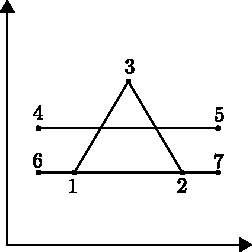
\includegraphics{./img/ch2-edgeint.pdf}
    \caption{The bunch of edges used for the tests.}
\end{figure}
@D planar\_arrangement support functions tests
@{@@testset "Edge fragmentation tests" begin
    V = [2 2; 4 2; 3 3.5; 1 3; 5 3; 1 2; 5 2]
    EV = sparse(Array{Int8, 2}([
        [1 1 0 0 0 0 0] #1->12
        [0 1 1 0 0 0 0] #2->23
        [1 0 1 0 0 0 0] #3->13
        [0 0 0 1 1 0 0] #4->45
        [0 0 0 0 0 1 1] #5->67
    ]))

    @@testset "intersect_edges" begin
        inters1 = intersect_edges(V, EV[5, :], EV[1, :])
        inters2 = intersect_edges(V, EV[1, :], EV[4, :])
        inters3 = intersect_edges(V, EV[1, :], EV[2, :])
        @@test inters1 == [([2. 2.], 1/4),([4. 2.], 3/4)]
        @@test inters2 == []
        @@test inters3 == [([4. 2.], 1)]
    end

    @@testset "frag_edge" begin
        rV, rEV = frag_edge(V, EV, 5)
        @@test rV == [2.0 2.0; 4.0 2.0; 3.0 3.5; 1.0 3.0; 
                     5.0 3.0; 1.0 2.0; 5.0 2.0; 2.0 2.0; 
                     4.0 2.0; 4.0 2.0; 2.0 2.0]
        @@test full(rEV) == [0 0 0 0 0 1 0 0 0 0 1; 
                            0 0 0 0 0 0 0 0 0 1 1;
                            0 0 0 0 0 0 1 0 0 1 0]
    end
end
@}









%%%%%%%%%%%%%%%%%%%%%%%%%%%%%%%%%%%
\section{Coincident vertices merge}
%++++++++++++++++++++++++++++%
\subsection{Support function}
\label{sec:merge_vertices}
The merge of coincident is done in the \texttt{merge\_vertices}
function. This relies on the \texttt{NearestNeighbors.jl} package\cite{NearestNeighbors}
which provides a reliable implementation of the \texttt{KDTree} data structure.
@D planar\_arrangement imports
@{using NearestNeighbors
@}
@D planar\_arrangement support functions
@{function merge_vertices(V::Verts, EV::Cells, err=1e-4)
    kdtree = KDTree(V')
    tocheck = collect(size(V,1):-1:1)
    todelete = Array{Int64, 1}()
    @< Iterate over tocheck @>
    @< Delete vertices in todelete @>
    @< Delete superfluous cells @>
    V,EV
end
@}
We create two stacks: \texttt{tocheck} which contains the indices of the vertices
to check and \texttt{todelete} that stores the indices of the vertices to delete later.
Into \texttt{tocheck} we put all the vertices of the complex in reverse order (in
this way we can pop from the stack the indices in crescent order). So, until \texttt{tocheck} is not empty,
we pop a vertex \texttt{vi} from the stack and for each coincident vertex \texttt{vj}, we put it 
into the \texttt{todelete} stack and we sum the columns of \texttt{EV} relative to \texttt{vi} and \texttt{vj}
@D Iterate over tocheck 
@{while !isempty(tocheck)
    vi = pop!(tocheck)
    if !(vi in todelete)
        nearvs = inrange(kdtree, V[vi, :], err)
        for vj in nearvs
            if vj != vi
                push!(todelete, vj)
                EV[:,vi] = EV[:, vi] + EV[:, vj]
            end
        end
    end
end
@}
We then calculate the vertices to keep and we filter out
the data relative to the vertices into \texttt{todelete}.
@D Delete vertices in todelete
@{tokeep = setdiff(collect(1:size(V,1)), todelete)
EV = EV[:, tokeep]
V = V[tokeep, :]
@}
At last we delete duplicated, empty and broken edges.
@D Delete superfluous cells
@{tokeep = Array{Int64, 1}()
cells = [Set(EV[i, :].nzind) for i in size(EV,1):-1:1]
i = 0
while !isempty(cells)
    i += 1
    c = pop!(cells)
    if !(length(c) != 2 || c in cells)
        push!(tokeep, i)
    end
end
EV = EV[tokeep, :]
@}
%+++++++++++++++++++++++++%
\subsection{Implementation}
We simply call \texttt{merge\_vertices} (ref. \ref{sec:merge_vertices}).
@D Merge coincident vertices
@{V, EV = merge_vertices(V, EV)
@}
%++++++++++++++++%
\subsection{Tests}
Let's merge the vertices of a square built by numerous
very similar edges.
@D planar\_arrangement support functions tests
@{@@testset "merge_vertices test set" begin
    n0 = 1e-12
    n1l = 1-1e-12
    n1u = 1+1e-12
    V = [ n0  n0; -n0  n0;  n0 -n0; -n0 -n0;
          n0 n1u; -n0 n1u;  n0 n1l; -n0 n1l;
         n1u n1u; n1l n1u; n1u n1l; n1l n1l;
         n1u  n0; n1l  n0; n1u -n0; n1l -n0]
    EV = Int8[1 0 0 0 1 0 0 0 0 0 0 0 0 0 0 0;
              0 1 0 0 0 1 0 0 0 0 0 0 0 0 0 0;
              0 0 1 0 0 0 1 0 0 0 0 0 0 0 0 0;
              0 0 0 1 0 0 0 1 0 0 0 0 0 0 0 0;
              0 0 0 0 1 0 0 0 1 0 0 0 0 0 0 0;
              0 0 0 0 0 1 0 0 0 1 0 0 0 0 0 0;
              0 0 0 0 0 0 1 0 0 0 1 0 0 0 0 0;
              0 0 0 0 0 0 0 1 0 0 0 1 0 0 0 0;
              0 0 0 0 0 0 0 0 1 0 0 0 1 0 0 0;
              0 0 0 0 0 0 0 0 0 1 0 0 0 1 0 0;
              0 0 0 0 0 0 0 0 0 0 1 0 0 0 1 0;
              0 0 0 0 0 0 0 0 0 0 0 1 0 0 0 1;
              1 0 0 0 0 0 0 0 0 0 0 0 1 0 0 0;
              0 1 0 0 0 0 0 0 0 0 0 0 0 1 0 0;
              0 0 1 0 0 0 0 0 0 0 0 0 0 0 1 0;
              0 0 0 1 0 0 0 0 0 0 0 0 0 0 0 1]
    EV = sparse(EV)
    V, EV = merge_vertices(V, EV)

    @@test V == [n0 n0; n0 n1u; n1u n1u; n1u n0]
    @@test full(EV) == [1 1 0 0;
                       0 1 1 0;
                       0 0 1 1;
                       1 0 0 1]
end
@}








%%%%%%%%%%%%%%%%%%%%%%%%%%%%%%%%%%%%%%%%
\section{Maximal biconnected components}
\begin{figure}[h]
    \centering
    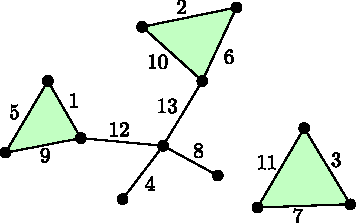
\includegraphics{./img/ch2-bicon.pdf}
    \caption{An example graph where the maximal biconnected 
    components are highlighted in green and the edges are numbered. 
    We have here three components formed by the sets of edges {1,5,9}, {2,6,10} and {3,11,7} }
    \label{img:bicon_comps}
\end{figure}
%+++++++++++++++++++++++++++%
\subsection{Support function}
\label{sec:biconnected_components}
To individuate the maximal biconnected components of the fragmented and merged 1-skeleton
we use the well know 1973 Hopcroft-Tarjan algorithm for biconnected components\cite{Hopcroft-Tarjan}.
@D planar\_arrangement support functions
@{function biconnected_components(EV::Cells)
    @< biconnected\_components local variables @>
    @< DFS utilities @>
    @< Depth first visit @>
    bicon_comps
end
@}
We will need a point stack (\texttt{ps}), an edge stack (\texttt{es}), a list of traversed edges (\texttt{todel}), a list of 
visited points (\texttt{visited}), a list of biconnected components (\texttt{bicon\_comps}) and a index to avoid duplicate 
numbering of vertices (\texttt{hivtx}). \texttt{ps} is made of triples composed by the index of the vertex in \texttt{V}, 
the index assigned by the algorithm and the component identifier also assigned by the algorithm. \texttt{es} instead 
contains couples with the index of the edge inside \texttt{EV} and the assigned index of the tail node. The indexes 
in \texttt{todel} and \texttt{bicon\_comps} are relative to \texttt{EV} while the ones of \texttt{visited} are
relative to \texttt{V}
@D biconnected\_components local variables
@{ps = Array{Tuple{Int, Int, Int}, 1}()
es = Array{Tuple{Int, Int}, 1}()
todel = Array{Int, 1}()
visited = Array{Int, 1}()
bicon_comps = Array{Array{Int, 1}, 1}()
hivtx = 1
@}
Here are implemented some functions helpful throughout the algorithm.
\texttt{an\_edge} returns the index relative to \texttt{EV} of the first edge out of \texttt{point} if exists or 
\texttt{false} otherwise. \texttt{get\_head}, given an \texttt{edge} and a point (the \texttt{tail}), returns the 
index relative to \texttt{V} of the head (the point that is not \texttt{tail}) of the \texttt{edge}. 
\texttt{v\_to\_vi}, given the index relative to \texttt{V} of a vertex (\texttt{v}), returns its index using 
the algorithm numbering. This index can also not exists; in this case \texttt{false} is returned.
@D DFS utilities
@{function an_edge(point)
    edges = setdiff(EV[:, point].nzind, todel)
    if length(edges) == 0
        edges = [false]
    end
    edges[1]
end

function get_head(edge, tail)
    setdiff(EV[edge, :].nzind, [tail])[1]
end

function v_to_vi(v)
    i = findfirst(t->t[1]==v, ps)
    if i == 0
        return false
    else
        return ps[i][2]
    end
end
@}
The DFS visit is mostly akin to the one proposed in the Hopcroft-Tarjan original algorithm.
The starting point is the first one in \texttt{V}.
@D Depth first visit
@{push!(ps, (1,1,1))
push!(visited, 1)
exit = false
while !exit
    edge = an_edge(ps[end][1])
    if edge != false
        tail = ps[end][2]
        head = get_head(edge, ps[end][1])
        hi = v_to_vi(head)
        if hi == false
            hivtx += 1
            push!(ps, (head, hivtx, ps[end][2]))
            push!(visited, head)
        else
            if hi < ps[end][3]
                ps[end] = (ps[end][1], ps[end][2], hi)
            end
        end
        push!(es, (edge, tail))
        push!(todel, edge)
    else
        if length(ps) == 1
            @< Handle disconnected graph @>
        else
            if ps[end][3] == ps[end-1][2]
                @< Form biconnected component @>
            else
                if ps[end-1][3] > ps[end][3]
                    ps[end-1] = (ps[end-1][1], ps[end-1][2], ps[end][3])
                end
            end
            pop!(ps)
        end
    end
end
@}
To form a biconnected component we pop edges out from the stack of edges (\texttt{es}) until we find the one
of which the index of its tail is equal to the component identifier (called \texttt{LOWPOINT} in the original algorithm) 
of the top point of the point stack (\texttt{ps}). We effectively put inside the \texttt{bicon\_comps} only the components
made of more than one edge because we are interested in building a 1-skeleton of valid 2-cells.
@D Form biconnected component
@{edges = Array{Int, 1}()
while true
    edge, tail = pop!(es)
    push!(edges, edge)
    if tail == ps[end][3]
        if length(edges) > 1
            push!(bicon_comps, edges)
        end
        break
    end
end
@}
When there are no more points to visit in the current connected component we search for a point in \texttt{V}
which has not been visited yet (so a point not listed in the \texttt{visited} array) and we put it on the top
of a new point stack and then let the algorithm iterate again. If there are no more new connected components 
to visit we break the algorithm iteration and exit.
@D Handle disconnected graph
@{found = false
pop!(ps)
for i in 1:size(EV,2)
    if !(i in visited)
        hivtx = 1
        push!(ps, (i, hivtx, 1))
        push!(visited, i)
        found = true
        break
    end
end
if !found
    exit = true
end
@}
%+++++++++++++++++++++++++%
\subsection{Implementation}
Like for the vertices merge we simply call the freshly implemented \texttt{biconnected\_components} function
(ref. \ref{sec:biconnected_components}). If no biconnected components are found, the procedure will stop and return nothing.
@D Find maximal biconnected components
@{bicon_comps = biconnected_components(EV)

if isempty(bicon_comps)
    println("No biconnected components found.")
    return
end
@}
We also need to delete edges that are not part of a maximal biconnected component
and then to delete the isolated vertices from both \texttt{V} and \texttt{EV}.
@D Filter biconnected components
@{todel = setdiff(collect(1:size(EV,1)), union(bicon_comps...))
EV = EV[union(bicon_comps...), :]

vertinds = 1:size(EV, 2)
todel = Array{Int64, 1}()
for i in vertinds
    if length(EV[:, i].nzind) == 0
        push!(todel, i)
    end
end
tokeep = setdiff(vertinds, todel)
EV = EV[:, tokeep]
V = V[tokeep, :]
@}
%++++++++++++++++%
\subsection{Tests}
The graph built here is the one of figure \ref{img:bicon_comps}.
@D planar\_arrangement support functions tests
@{@@testset "biconnected_components test set" begin
    EV = Int8[0 0 0 1 0 0 0 0 0 0 1 0; #1
              0 0 1 0 0 1 0 0 0 0 0 0; #2
              0 0 0 0 0 0 1 0 0 1 0 0; #3
              1 0 0 0 1 0 0 0 0 0 0 0; #4
              0 0 0 1 0 0 0 1 0 0 0 0; #5
              0 0 1 0 0 0 0 0 1 0 0 0; #6
              0 1 0 0 0 0 0 0 0 1 0 0; #7
              0 0 0 0 1 0 0 0 0 0 0 1; #8
              0 0 0 0 0 0 0 1 0 0 1 0; #9
              0 0 0 0 0 1 0 0 1 0 0 0; #10
              0 1 0 0 0 0 1 0 0 0 0 0; #11
              0 0 0 0 1 0 0 0 0 0 1 0; #12
              0 0 0 0 1 0 0 0 1 0 0 0] #13
    EV = sparse(EV)

    bc = biconnected_components(EV)
    bc = Set(map(Set, bc))

    @@test bc == Set([Set([1,5,9]), Set([2,6,10]), Set([3,7,11])])
end
@}













%%%%%%%%%%%%%%%%%%%%%%%%
\section{Faces creation}
%+++++++++++++++++++++++++%
\subsection{Implementation}
@D Create faces
@{bicon_comps = biconnected_components(EV)

n = size(bicon_comps, 1)
shells = Array{Cell, 1}(n)
boundaries = Array{Cells, 1}(n)
EVs = Array{Cells, 1}(n)
for p in 1:n
    ev = EV[bicon_comps[p], :]
    fe = minimal_2cycles(V, ev)
    shell_num = get_external_cycle(V, ev, fe)

    EVs[p] = ev 
    tokeep = setdiff(1:fe.m, shell_num)
    boundaries[p] = fe[tokeep, :]
    shells[p] = fe[shell_num, :]
end

@< Containment test @>
@< Transitive reduction @>
@< Cell merging @>

@}

@D planar\_arrangement imports
@{include("./minimal_cycles.jl")
@}

%++++++++++++++++++++++++++++++++++++++++%
\subsection{Individuate the external cell}
Once we computed the minimal 2-cycles (ref. \ref{ch:minimal_cycles})
we need to individuate the external cycle. To do this we iterate over the
vertices of the passed \texttt{EV} to find four vertices: the two with biggest
$x_1$ and $x_2$ coordinates (\texttt{maxv\_x1} and \texttt{maxv\_x2}) and the 
two with the smallest one (\texttt{minv\_x1} and \texttt{minv\_x2}). 
Then we check which face the two vertices have in common. 

It can happen that the two vertices have more than one face in common
(for example when a biconnected component is made up only by one face);
in this case we simply pick the cell with negative area. The area
computation routines are located into Chapter 5 (ref. \ref{sec:face_area})


@D planar\_arrangement support functions
@{function get_external_cycle(V::Verts, EV::Cells, FE::Cells)
    FV = abs(FE)*EV
    vs = sparsevec(mapslices(sum, abs(EV), 1)).nzind
    minv_x1 = maxv_x1 = minv_x2 = maxv_x2 = pop!(vs)
    for i in vs
        if V[i, 1] > V[maxv_x1, 1]
            maxv_x1 = i
        elseif V[i, 1] < V[minv_x1, 1]
            minv_x1 = i
        end
        if V[i, 2] > V[maxv_x2, 2]
            maxv_x2 = i
        elseif V[i, 2] < V[minv_x2, 2]
            minv_x2 = i
        end
    end
    cells = intersect(
        FV[:, minv_x1].nzind, 
        FV[:, maxv_x1].nzind,
        FV[:, minv_x2].nzind,
        FV[:, maxv_x2].nzind
    )
    if length(cells) == 1
        return cells[1]
    else
        for c in cells
            if face_area(V, EV, FE[c, :]) < 0
                return c
            end
        end
    end
end
@}

%+++++++++++++++++++++++++++%
\subsection{Containment test}

For each shell we must compute if it is contained
in another shell. So, for every couple of shells
we must check if one is contained into the other.
This check must be performed by shooting a ray from
a vertex of the first cell and then count the intersections
of it with the edges of the second cell; if the number 
of the intersections is odd then the first cell is contained
in the second one. This computation is rather heavy but can be
speeded up by pre-computing an approximate containment graph 
using a bounding box containment test. Then the graph must be
pruned shooting a ray for every arc of it. In this way we reduce
considerably the amount of rays we shoot. (This is also visually
explained in the tests: ref. \ref{sec:conttest_test})

Before building the containment graph, we
compute the bounding boxes of the shells and we store them into
the \texttt{shell\_bboxes} list (we are going to use this also later).
The bounding box logic is implemented in the utilities of chapter 5 
(ref. \ref{sec:bboxes})

@D Containment test
@{shell_bboxes = []
for i in 1:n
    vs_indexes = (abs(EVs[i]')*abs(shells[i])).nzind
    push!(shell_bboxes, bbox(V[vs_indexes, :]))
end

containment_graph = pre_containment_test(shell_bboxes)
containment_graph = prune_containment_graph(n, V, EVs, shells, containment_graph)
@}

@D planar\_arrangement support functions
@{function pre_containment_test(bboxes)
    n = length(bboxes)
    containment_graph = spzeros(Int8, n, n)

    for i in 1:n
        for j in 1:n
            if i != j && bbox_contains(bboxes[j], bboxes[i])
                containment_graph[i, j] = 1
            end
        end
    end

    return containment_graph
end
@}

The ray logic is explained just below the next macro.

@D planar\_arrangement support functions
@{function prune_containment_graph(n, V, EVs, shells, graph)
    
    for i in 1:n
        an_edge = shells[i].nzind[1]
        origin_index = EVs[i][an_edge, :].nzind[1]
        origin = V[origin_index, :]
 
        for j in 1:n
            if i != j
                if graph[i, j] == 1
                    contains = false
                    @< Shoot ray @>
                    if !contains
                        graph[i, j] = 0
                    end
                end
             end
         end

     end
     return graph
end
@}

We shoot a ray from the vertex $o$ with the same direction
of the positive $x_1$ semi-axis.
When we want to find the intersection of the ray with an edge,
we parametrize it:

\begin{equation}
\label{eq:edge}
    p = p_1 + \alpha(p_2-p_1), \quad\alpha\in[0, 1]
\end{equation}

Then we find the value that $\alpha$ assumes when the edge
intersects the line parallel to the $x_1$ axis that passes through $o$:

\begin{gather*}
    \begin{bmatrix}
        o_x \\ o_y
    \end{bmatrix}
    = 
    \begin{bmatrix}
        p_{1x} \\ p_{1y}
    \end{bmatrix}
    +
    \alpha
    \begin{bmatrix}
        p_{2x} - p_{1x} \\ p_{2y} - p_{1y}
    \end{bmatrix} \\
    o_y = p_{1y} + \alpha(p_{2y} - p_{1y}) \\
    \alpha = \frac{o_y - p_{1y}}{p_{2y} - p_{1y}}
\end{gather*}

If $\alpha\in[0, 1]$ then the edge intersect the line, and we find the point
of intersection by putting $\alpha$ into equation \ref{eq:edge}.
The intersection must be count only if the freshly computed point
is on the right of the vertex $o$.

The case when the ray encounters a vertex requires additional care:
we are testing the intersections of the ray with edges, and every
vertex is shared by two or more edges. So we cannot simply increase the 
\texttt{hits} counter every time we encounter a vertex because this will lead
to miscalculations when an even number of edges share the same vertex.
We resolve this by storing the already visited vertices into the 
\texttt{visited\_verts} list.

@D Shoot ray
@{hits = 0
visited_verts = []
shell_edge_indexes = shells[j].nzind
ev = EVs[j][shell_edge_indexes, :]

for edge in 1:ev.m
    a_id, b_id = ev[edge, :].nzind
    a = V[a_id, :]
    b = V[b_id, :]
    v = b - a
    alpha = (origin[2] - a[2]) / v[2]
    if 0 <= alpha <= 1
        x_int = a[1] + v[1]*alpha
        if x_int > origin[1]
            if 0 <= alpha <= 1
                hits += 1
            else
                p = (alpha == 0) ? a : b
                if !(p in visited_verts)
                    hits += 1
                    push!(visited_verts, p)
                end
            end
        end
    end
end

contains = hits % 2 == 1
@}


%+++++++++++++++++++++++++++++++%
\subsection{Transitive reduction}

We have an adjacency matrix and we must perform a transitive reduction.
As explained by A. V. Aho, M. R. Garey, and J. D. Ullman \cite{parallel_transitive_reduction}
we have:

@D Transitive reduction
@{transitive_reduction!(containment_graph) 
@}

@D planar\_arrangement support functions
@{function transitive_reduction!(graph)
    n = size(graph, 1)
    for j in 1:n
        for i in 1:n
            if graph[i, j] > 0
                for k in 1:n
                    if graph[j, k] > 0
                        graph[i, k] = 0
                    end
                end
            end
        end
    end
end
@}

%+++++++++++++++++++++++%
\subsection{Cell merging}

For every arc of the containment tree we have a father component 
and a child component and we must find the cycle of the father that
contains the child. This happens if the bounding box of the child is fully
contained in the box of the cycle. The bounding box logic is implemented
in the utilities of chapter 5 (ref. \ref{sec:bboxes}, please note that
that the \texttt{bboxes} is not part of the utilities but it is defined 
in the next paragraph). The \texttt{sums} array contains the indexes of 
the rows of the various boundary matrices to sum after the containment 
graph has been traversed. Every element is a triple made of: the father 
index, the father's container cell index and the child index.
Once we individuated the rows to sum, we actually need to perform the sum.
This is non trivial because we must build the final boundary matrix.
These computations are delegated to the $\langle$ Create EV and FE $\rangle$ macro.
@D Cell merging 
@{EV, FE = cell_merging(n, containment_graph, V, EVs, boundaries, shells, shell_bboxes)
@}

@D planar\_arrangement support functions 
@{function cell_merging(n, containment_graph, V, EVs, boundaries, shells, shell_bboxes)
    @< Cell merging support functions @>

    sums = Array{Tuple{Int, Int, Int}}(0);

    for father in 1:n
        if sum(containment_graph[:, father]) > 0
            father_bboxes = bboxes(V, abs(EVs[father]')*abs(boundaries[father]'))
            for child in 1:n
                if containment_graph[child, father] > 0
                    child_bbox = shell_bboxes[child]
                    for b in 1:length(father_bboxes)
                        if bbox_contains(father_bboxes[b], child_bbox)
                            push!(sums, (father, b, child))
                            break
                        end
                    end
                end            
            end
        end
    end

    @< Create EV and FE @>
    return EV, FE
end
@}

The \texttt{bboxes} computes the bounding boxes of each cycle
described in the \texttt{indexes} matrix.

@D Cell merging support functions
@{function bboxes(V::Verts, indexes::Cells)
    boxes = Array{Tuple{Any, Any}}(indexes.n)
    for i in 1:indexes.n
        v_inds = indexes[:, i].nzind
        boxes[i] = bbox(V[v_inds, :])
    end
    boxes
end
@}

To actually build the complete and correct boundary matrix \texttt{FE},
we compute the final dimensions of it, then we initialize it filled with
zeros and then we fill it with the correct data in the correct position.
While doing this we store into \texttt{c\_offsets} the column offset of each
biconnected component; we will use this information to quickly find the columns 
to sum from the \texttt{sums} array of triples.

@D Create EV and FE
@{EV = vcat(EVs...)
edgenum = size(EV, 1)
facenum = sum(map(x->size(x,1), boundaries))
FE = spzeros(Int8, facenum, edgenum)
shells2 = spzeros(Int8, length(shells), edgenum)
r_offsets = [1]
c_offset = 1
for i in 1:n
    min_row = r_offsets[end]
    max_row = r_offsets[end] + size(boundaries[i], 1) - 1
    min_col = c_offset
    max_col = c_offset + size(boundaries[i], 2) - 1
    FE[min_row:max_row, min_col:max_col] = boundaries[i]
    shells2[i, min_col:max_col] = shells[i]
    push!(r_offsets, max_row + 1)
    c_offset = max_col + 1
end

for (f, r, c) in sums
    FE[r_offsets[f]+r-1, :] += shells2[c, :]
end
@}


%++++++++++++++++%
\subsection{Tests}

@D planar\_arrangement support functions tests
@{@@testset "Face creation" begin
    @< Face creation tests @>
end
@}

\subsubsection{External cell individuation}
\begin{figure}[h]
    \centering
    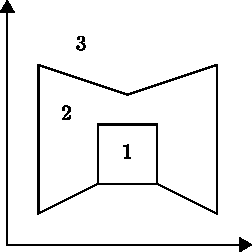
\includegraphics{./img/ch2-externcell.pdf}
    \caption{This biconnected component has three faces. The external one is the number 3.
    This is a particularly difficult case because the most "external" vertices of face 2
    are in common with the external cell.}
\end{figure}

@D Face creation tests
@{@@testset "External cell individuation" begin
    V = [ .5 .5;  1.5   1;  1.5  2; 
         2.5  2;  2.5   1;  3.5 .5;
         3.5  3;    2 2.5;   .5  3]

    EV = Int8[-1  1  0  0  0  0  0  0  0;
               0 -1  1  0  0  0  0  0  0;
               0  0 -1  1  0  0  0  0  0;
               0  0  0 -1  1  0  0  0  0;
               0  0  0  0 -1  1  0  0  0;
               0  0  0  0  0 -1  1  0  0;
               0  0  0  0  0  0 -1  1  0;
               0  0  0  0  0  0  0 -1  1;
              -1  0  0  0  0  0  0  0  1;
               0 -1  0  0  1  0  0  0  0]
    EV = sparse(EV)
    
    FE = Int8[ 0 -1 -1 -1  0  0  0  0  0  1;
               1  1  1  1  1  1  1  1 -1  0;
              -1  0  0  0 -1 -1 -1 -1  1 -1]
    FE = sparse(FE)

    @@test get_external_cycle(V, EV, FE) == 3
end
@}

\subsubsection{Containment test}
\label{sec:conttest_test}

\begin{figure}[h]
    \centering
    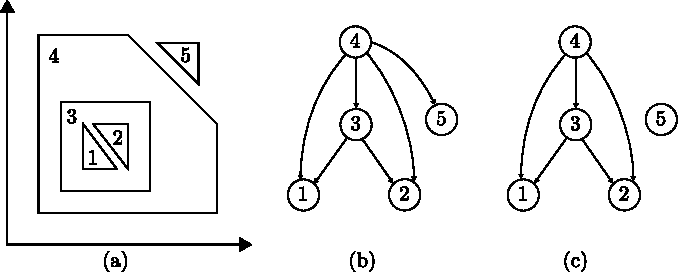
\includegraphics{./img/ch2-containmenttest.pdf}
    \caption{(a) is our test case. The numbers identify the connected components. 
        (b) is the containment graph built using only the \texttt{pre\_containment\_test} 
        function. The arc (4,5) is in there because the bounding box of the component 
        no. 5 is completely contained in the bounding box of no. 4. (c) shows 
        the graph after the \texttt{prune\_containment\_graph} function.}
\end{figure}

@D Face creation tests
@{@@testset "Containment test" begin
    V = [  0   0;    4   0;    4   2;   2   4;  0 4;
          .5  .5;  2.5  .5;  2.5 2.5;  .5 2.5;
           1   1;  1.5   1;    1   2;
           2   1;    2   2;  1.5   2;
         3.5 3.5;    3 3.5;  3.5   3]
    EV1 = Int8[ 0  0  0  0  0  0  0  0  0 -1  1  0  0  0  0  0  0  0;
                0  0  0  0  0  0  0  0  0  0 -1  1  0  0  0  0  0  0;
                0  0  0  0  0  0  0  0  0 -1  0  1  0  0  0  0  0  0]
    EV2 = Int8[ 0  0  0  0  0  0  0  0  0  0  0  0 -1  1  0  0  0  0;
                0  0  0  0  0  0  0  0  0  0  0  0  0 -1  1  0  0  0;
                0  0  0  0  0  0  0  0  0  0  0  0 -1  0  1  0  0  0]
    EV3 = Int8[ 0  0  0  0  0 -1  1  0  0  0  0  0  0  0  0  0  0  0;
                0  0  0  0  0  0 -1  1  0  0  0  0  0  0  0  0  0  0;
                0  0  0  0  0  0  0 -1  1  0  0  0  0  0  0  0  0  0;
                0  0  0  0  0 -1  0  0  1  0  0  0  0  0  0  0  0  0]
    EV4 = Int8[-1  1  0  0  0  0  0  0  0  0  0  0  0  0  0  0  0  0;
                0 -1  1  0  0  0  0  0  0  0  0  0  0  0  0  0  0  0;
                0  0 -1  1  0  0  0  0  0  0  0  0  0  0  0  0  0  0;
                0  0  0 -1  1  0  0  0  0  0  0  0  0  0  0  0  0  0;
               -1  0  0  0  1  0  0  0  0  0  0  0  0  0  0  0  0  0]
    EV5 = Int8[ 0  0  0  0  0  0  0  0  0  0  0  0  0  0  0 -1  1  0;
                0  0  0  0  0  0  0  0  0  0  0  0  0  0  0  0 -1  1;
                0  0  0  0  0  0  0  0  0  0  0  0  0  0  0 -1  0  1]
    EVs = map(sparse, [EV1, EV2, EV3, EV4, EV5])
    
    shell1 = Int8[-1 -1  1];
    shell2 = Int8[-1 -1  1];
    shell3 = Int8[-1 -1 -1  1];
    shell4 = Int8[-1 -1 -1 -1  1];
    shell5 = Int8[-1 -1  1];
    shells = map(sparsevec, [shell1, shell2, shell3, shell4, shell5])
    
    shell_bboxes = []
    n = 5
    for i in 1:n
        vs_indexes = (abs(EVs[i]')*abs(shells[i])).nzind
        push!(shell_bboxes, bbox(V[vs_indexes, :]))
    end

    graph = pre_containment_test(shell_bboxes)
    @@test graph == [0 0 1 1 0; 0 0 1 1 0; 0 0 0 1 0; 0 0 0 0 0; 0 0 0 1 0]

    graph = prune_containment_graph(n, V, EVs, shells, graph)
    @@test graph == [0 0 1 1 0; 0 0 1 1 0; 0 0 0 1 0; 0 0 0 0 0; 0 0 0 0 0]
end
@}

\subsubsection{Transitive reduction}
\label{sec:transitivered_test}

\begin{figure}[h]
    \centering
    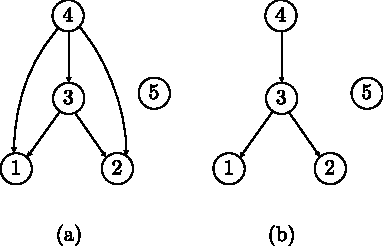
\includegraphics{./img/ch2-transitivered.pdf}
    \caption{Before (a) and after (b) transitive reduction performed on
    the graph of the previous test set.}
\end{figure}

@D Face creation tests
@{@@testset "Transitive reduction" begin
    graph = [0 0 1 1 0; 0 0 1 1 0; 0 0 0 1 0; 0 0 0 0 0; 0 0 0 0 0]
    transitive_reduction!(graph)
    @@test graph == [0 0 1 0 0; 0 0 1 0 0; 0 0 0 1 0; 0 0 0 0 0; 0 0 0 0 0]
end
@}

\subsubsection{Cell merging}

\begin{figure}[h]
    \centering
    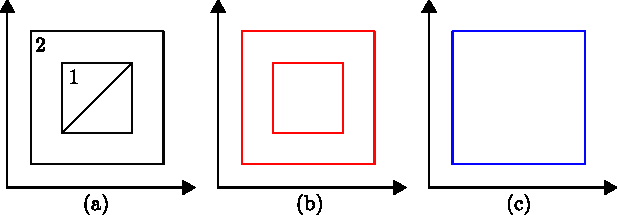
\includegraphics{./img/ch2-cellmerge.pdf}
    \caption{Here we have two biconnected components, one inside the other (a).
    If we don't perform cell merging, the boundary of the arranged set will be
    the red one (b), which is incorrect. The correct boundary is the blue one (c).}
\end{figure}

@D Face creation tests
@{@@testset "Cell merging" begin
    graph = [0 1; 0 0]
    V = [.25 .25; .75 .25; .75 .75; .25 .75;
           0   0;   1   0;   1   1;   0   1]
    EV1 = Int8[-1  1  0  0  0  0  0  0;
                0 -1  1  0  0  0  0  0;
                0  0 -1  1  0  0  0  0;
               -1  0  0  1  0  0  0  0;
               -1  0  1  0  0  0  0  0]
    EV2 = Int8[ 0  0  0  0 -1  1  0  0;
                0  0  0  0  0 -1  1  0;
                0  0  0  0  0  0 -1  1;
                0  0  0  0 -1  0  0  1]
    EVs = map(sparse, [EV1, EV2])

    shell1 = Int8[-1 -1 -1  1  0]
    shell2 = Int8[-1 -1 -1  1]
    shells = map(sparsevec, [shell1, shell2])

    boundary1 = Int8[ 1  1  0  0 -1;
                      0  0  1 -1  1]
    boundary2 = Int8[ 1  1  1 -1]
    boundaries = map(sparse, [boundary1, boundary2])

    shell_bboxes = []
    n = 2
    for i in 1:n
        vs_indexes = (abs(EVs[i]')*abs(shells[i])).nzind
        push!(shell_bboxes, bbox(V[vs_indexes, :]))
    end

    EV, FE = cell_merging(2, graph, V, EVs, boundaries, shells, shell_bboxes)

    selector = sparse(ones(Int8, 1, 3))

    @@test selector*FE == [0  0  0  0  0  1  1  1 -1]
end
@}